After presenting the main results, and its analysis, in this section we discuss some details of our studies, including the threats to their validity.
%In conducting the different studies, we have found that there is a great variety in the testability of the different projects, even within the same study. In this section we will discuss the semantics of the testability metrics, analyse some of the projects with the higher testability, study why projects have low testability and, finally, present the  threats to validity of this work.

\michel{Aqui faltan dos subsecciones: una sobre la semantica de las metricas, y otra sobre los proyectos con alta testabilidad. La primera queda bastante obsoleta con el CaseStudy, la segunda tendría que volver a escribirla, ya que las métricas no son las mismas}

% \subsection{On the semantics of testability metrics}
% \label{sec:semantics}

% \michel{Es posible que esta sub-sección, con el nuevo Case Study, no tenga mucho sentido}

% For the studies presented in this paper, we designed a framework based on extending compilability to consider also compilability of tests, and introducing four \textit{Testability} metrics. 
% Each of these metrics shows a different aspect of testability.

% In continuous integration systems it is common that all tests must pass, being the result of their execution a binary value: either all tests pass or all tests fail. 
% In this context, we define that a commit is Fully Testable if all tests are success. 
% At the project level, we can identify how many commits are Fully Testable and provide a metric representing their percentage (Fully Testability). 
% It is common to consider all the commits of a project to calculate this type of metric.
% \textit{Fully Testability\textsubscript{A}} could be considered the ``absolute'' testability, since it considers all commits.
% In a project with 100\% \textit{Fully Testability\textsubscript{A}} all past snapshots are testable. 
% However, there are constraints, not related to the tests themselves, that put limits to testability.
% For example, a test that cannot be built, cannot be run. 
% Therefore, we defined \textit{Fully Testability\textsubscript{T}} to capture these constraints, and define testability related to them. 
% They inform on the quality of the tests only for snapshots that are compilable (either source- and tests-compilable). 
% In more detail:

% \begin{itemize}
%     \item \textbf{A high \textit{Fully Testability\textsubscript{A}}} signals a \textbf{highly reproducible project}: most of its snapshots are compilable, and the execution of their tests is successful.
%     The project in our dataset with the highest value in this metric is \textit{jsoup}, with a value of 93.55\%. 
%     This project, and others with high \textit{Fully Testability\textsubscript{A}}, are analyzed in the section~\ref{sec:high}.
%     \item \textbf{A high \textit{Fully Testability\textsubscript{T}}} hints to a project with \textbf{highly reproducible execution of tests}: most tests that can be built can also be executed successfully. 
%     A good example is \textit{JFinal}, with a value of 100\%. 
%     Its low \textit{Test Compilability} (22\%) considerably affects its \textit{Fully Testability\textsubscript{B}} (22\%). 
%     In this case, \textit{Fully Testability\textsubscript{T}} shows that as long as the tests are built correctly, they can be executed successfully. 
%     In projects with high \textit{Fully Testability\textsubscript{T}} and low \textit{Test Compilability} it is reasonable to think that improving \textit{Test Compilability} could increase also \textit{Fully Testability\textsubscript{A}}.
% \end{itemize}

% There are some projects as well with a high percentage of tests executed successfully, but low \textit{Fully Testability}. 
% This is possible when many tests in a snapshot are executed successfully, but a few do not. 
% For example, Figure~\ref{fig:checkstyle} shows a stacked area chart of the test results for all snapshots of \textit{Checkstyle}: snapshots are in the X axis, and the number of tests for each of them in the Y axis. Most of the tests for each snapshot are green (test success), but there is a small orange area close to the X axis corresponding to tests executed with error. 
% Due to these errors, most of the commits are not testable, and the project has a very low \textit{Fully Testability\textsubscript{A}} (1\%). 
% The reason for this is binary definition for Fully Testability, based on the rule of ``all tests should pass''. 
% Even when it is useful to compare with the ideal situation, there is room for defining additional metrics that reflect the high reproducibility of the tests in projects like this.

% \begin{figure}[t]
%     \centering    
%     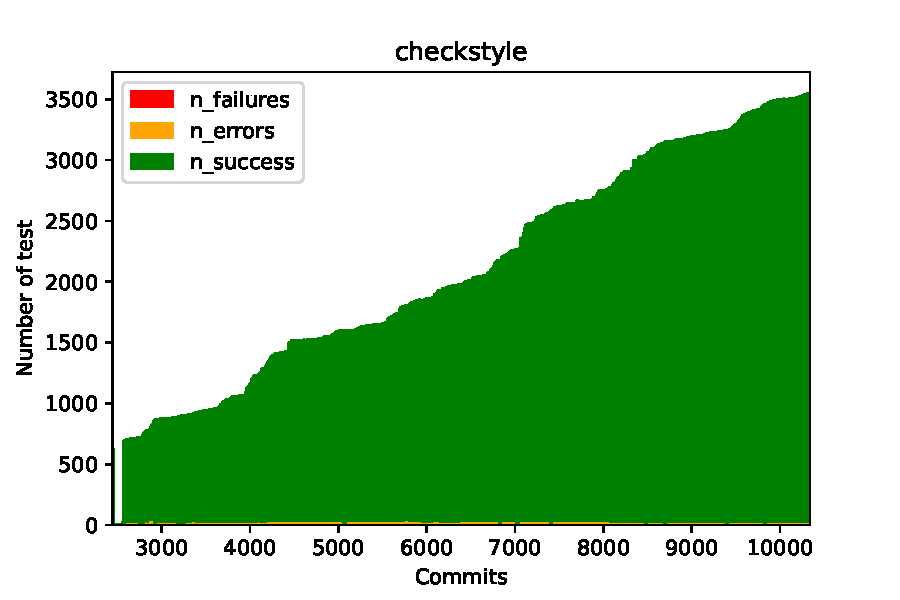
\includegraphics[width=8cm]{images/checkstyle.pdf}
%     \vspace{-0.2cm}
%     \caption{Tests results for Checkstyle project}
%     \label{fig:checkstyle}
% \end{figure}

% For this purpose, for each project commit, we define \textit{Testable Rate}. 
% This value will show us the ratio of tests with a success result against the total number of tests of that commit. 
% In this way, \textit{Testable Rate} gives us a more complete view of how the tests have behaved in a commit.
% Thus, a commit being \textit{Fully Testable} would only be a particular case where the value of \textit{Testable Rate} is 100\%.

% In order to study the percentage of tests that pass at the project level, we find that it is difficult to capture in a metric that clearly reflects how the tests behave in the commit history. 
% The main limitation is when we consider all commits, since in those where the source code or test code cannot be built, we assume a Testable Rate of 0\% because we do not know the real Testable Rate.

% To illustrate it in an example, in Figure~\ref{fig:closure} we see the result of the tests in the history of the Closure project. 
% Several commits on its commit history cannot be built. 
% The mean Testable Rate of all its commits is 59\%, while the median reaches 100\%.
% As in Fully Testability, in order to deal with the limitations of project compilability, Testability Rate C, B and T, considering all commits, source-compilable and test-compilable commits respectively, are defined in an analogous way.

% \begin{figure}[h]
%     \centering    
%     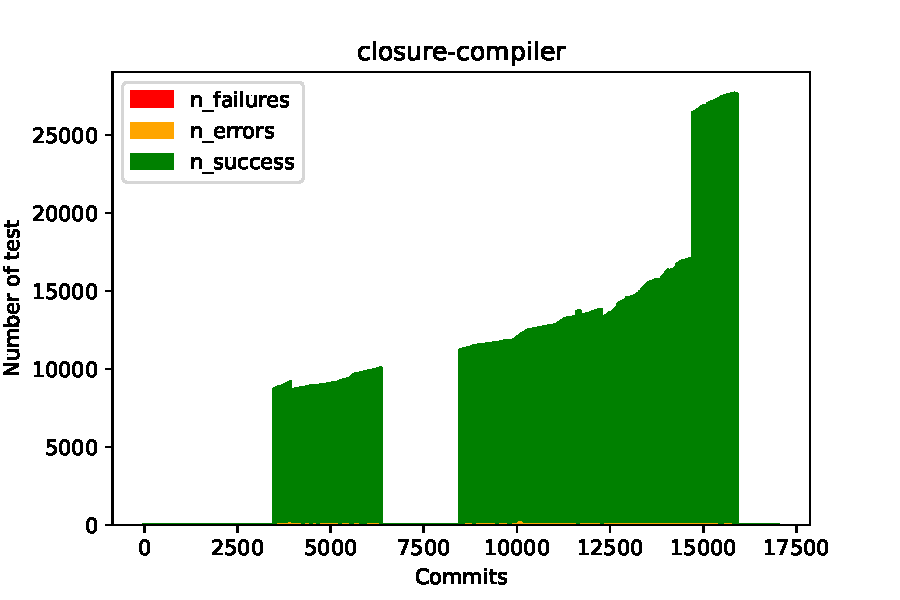
\includegraphics[width=8cm]{images/Closure.pdf}
%     \vspace{-0.2cm}
%     \caption{Tests results for Closure Compiler project}
%     \label{fig:closure}
% \end{figure}

% \subsection{Projects with high testability}
% \label{sec:high}

% We have identified some projects with high testability, which deserve a separate analysis. 
% To show these cases, we have searched for projects with the highest \textit{TestabilitRate} and the highest \textit{Fully Testability}.

% After analyzing the Testability Rate of the projects, we wanted to check which projects offer the highest results. Of the 86 projects:
% \begin{itemize}
%     \item We found 11 where the Testability Rate\textsubscript{A} is 100\% (i.e. in at least 50\% of their commits all the tests pass).
%     \item We found 39 where the Testability Rate\textsubscript{B} is 100\% (i.e. in at least 50\% of their source-compilable commits all the tests pass).
%     \item We found 44 where the Testability Rate\textsubscript{T} is 100\% (i.e. in at least 50\% of their test-compilable commits all the tests pass).
% \end{itemize}

% These values give us a very high number of projects, making an in-depth analysis difficult. 
% Therefore, in order to study projects with high testability, we have limited to those with high Fully Testability. 
% Specifically, we have selected the 3 projects that offer the best results for the different variants of Fully Testability (C, B and T).

% Tables~\ref{table:high-testability-A} and~\ref{table:high-testability-T} show metrics of the three projects with the highest Fully Testability of each flavor (A and T). 
% % La siguiente frase necesitaria más desarrollo
% %They could be good for identifying good practices that may help to increase testability of other projects.

% \begin{table}[h]
%     \centering
%     \caption{Top three projects with the highest \textit{Fully Testability\textsubscript{A}}}
%     \label{table:high-testability-A}
    
%     \begin{tabular}{|r|r|r|r|}
%         \hline
%         \textbf{Project}                  & \textbf{jsoup} & \textbf{spark} & \textbf{retrofit} \\ \hline
%         \textbf{Age}                      & 11.12          & 9.54           & 10.47         \\ \hline
%         \textbf{LoC}                      & 17,831         & 8,655          & 22,003           \\ \hline
%         \textbf{Total Commits}            & 1,442          & 1,062          & 1,865              \\ \hline
%         \textbf{Source-compilable commits} & 1,410          & 1,051          & 1,431              \\ \hline
%         \textbf{Source compilability}      & 0.97           & 0.98           & 0.76          \\ \hline
%         \textbf{Test-compilable commits}   & 1,403          & 986            & 1,431              \\ \hline
%         \textbf{Test compilability}        & 0.99           & 0.93           & 1.0               \\ \hline
%         \textbf{Fully Testable commits}    & 1349           & 921            & 1,411              \\ \hline
%         \textbf{Fully Testability\textsubscript{A}}      & \textbf{0.93} & \textbf{0.86} & \textbf{0.75} \\ \hline
%         \textbf{Fully Testability\textsubscript{B}}      & 0.95           & 0.87           & 0.98          \\ \hline
%         \textbf{Fully Testability\textsubscript{T}}      & 0.96           & 0.93           & 0.98          \\ \hline
%         \textbf{Testability Rate\textsubscript{A}}       & 1.0            & 1.0            & 1.0               \\ \hline
%         \textbf{Testability Rate\textsubscript{B}}       & 1.0            & 1.0            & 1.0               \\ \hline
%         \textbf{Testability Rate\textsubscript{T}}       & 1.0            & 1.0            & 1.0               \\ \hline
%     \end{tabular}
% \end{table}

% Among the projects with a high \textit{Fully Testability\textsubscript{A}} is \textit{jsoup}, a popular programming library for manipulating HTML code, which has only unit and integration tests.
% The second project, \textit{retrofit}, is a simple HTTP client, with the particularity that it is a multi-module project. 
% A high t\textit{Fully Testability\textsubscript{A}} C indicates that the tests of all its modules pass completely in most of the commits.
% All its tests use mocks, defined in its own module. 
% The robustness of testing functionality with mocks rather than with real endpoints (subject to change over time) may be one of the reasons for the good results of this project in this metric.
% The third project, \textit{spark}, is a lightweight web development framework. 
% It has end-to-end tests to verify the correct behavior when HTTP requests are performed; we have observed that these requests do not depend on remote services, though, which we have found in other projects to be a reason for low testability (see Section~\ref{sec:low-testability}).

% \begin{table}[h]
%     \centering
%     \caption{Top three projects with the highest \textit{Fully Testability\textsubscript{T}}}
%     \label{table:high-testability-T}
%     \begin{tabular}{|r|r|r|r|}
%         \hline
%         \textbf{Project}                  & \textbf{otto} & \textbf{javapoet} & \textbf{camel} \\ \hline
%         \textbf{Age}                      & 5.85          & 8.88              & 14.28          \\ \hline
%         \textbf{LoC}                      & 1,344        & 8,306            & 1,146,447      \\ \hline
%         \textbf{Total Commits}            & 205           & 846               & 53,286          \\ \hline
%         \textbf{Source-compilable commits} & 18            & 398               & 21             \\ \hline
%         \textbf{Source compilability}      & 0.09          & 0.47              & 0.0            \\ \hline
%         \textbf{Test-compilable commits}   & 18            & 396               & 20             \\ \hline
%         \textbf{Test compilability}        & 1.0           & 0.99              & 0.95           \\ \hline
%         \textbf{Fully Testable commits}   & 18            & 396               & 20             \\ \hline
%         \textbf{Fully Testability\textsubscript{A}}      & 0.09          & 0.47              & 0.0            \\ \hline
%         \textbf{Fully Testability\textsubscript{B}}      & 1.0           & 0.99              & 0.95           \\ \hline
%         \textbf{Fully Testability\textsubscript{T}}      & \textbf{1.0}  & \textbf{1.0}      & \textbf{1.0}   \\ \hline
%         \textbf{Testability Rate\textsubscript{A}}       & 0.0           & 0.0               & 0.0            \\ \hline
%         \textbf{Testability Rate\textsubscript{B}}       & 1.0           & 1.0               & 1.0            \\ \hline
%         \textbf{Testability Rate\textsubscript{T}}       & 1.0           & 1.0               & 1.0            \\ \hline
%     \end{tabular}
% \end{table}

% The three projects selected for the table with the highest \textit{Fully Testability\textsubscript{T}} are particularly interesting: whenever their tests could be constructed, they could be executed successfully. Two of them appeared in previous tables (\textit{otto} and \textit{javapoet}). The \textit{camel} project (a service integration library) offers a high \textit{Fully Testability\textsubscript{T}}, but this result must be considered in view of the fact that its compilability is only 0.03\%. For projects like this it is important to consider all \textit{Fully Testability} variants. 

\subsection{Why do projects have low testability?}
\label{sec:low-testability}

We have performed a preliminary study to identify the main reasons for some projects having low Fully Testability\textsubscript{A}. 
These reasons can be organized in three types:

\subsubsection{Low compilability.} 

\textit{Fully Testability\textsubscript{A}} of a project depends on the steps prior to the execution of the tests: compiling the main source code and the tests.
In projects with low compilability, testability is constrained by it.
Tufano et al. showed how one of the main reasons why a commit is no longer compilable is because of an error in obtaining the project dependencies~\cite{tufano2017there}. 
Therefore, it is possible that if those dependencies were available, the project not only built correctly, but also its tests could be executed successfully. 
We found several projects where the \textit{Fully Testability\textsubscript{A}} is low due to low compilability, but \textit{Fully Testability\textsubscript{T}} is high, which is in line with this hypothesis.

\subsubsection{Snapshots were never testable.} When the project was being developed, not all of its commits were testable:

\begin{itemize}
    \item  \textbf{No tests in the snapshot}: 
    In some projects we have found no tests for some commits. 
    We consider these commits without test as non-testable, resulting in low values if many snapshots are like that.
    In these cases, the project may not have developed the tests in the early stages of development.
    \item \textbf{Snapshots with failing tests}: 
    When compiling and running tests on snapshots, we decided to try all of them in the master branch, since a recent study by Kovalenko et al.~\cite{kovalenko:2018:miningfilehistories} has shown that considering additional branches does not seem to have a significant impact compared to using only the master branch. 
    But depending on the strategy used by the developers to merge changes into master, we may find commits with tests failing even when they were merged. 
    For example, a commit includes a new feature which breaks some tests, but it is still merged, maybe because the next commit will fix the tests or the cause of the error.
    We found this case in \textit{elastic-job} project by taking advantage of commit comments to understand the development workflow. 
    When refactoring, tests stop passing in some commits, being fixed in later commits (for example see commits 860, 929, 965, 1053 and 1120, where 0 is the last commit in the history).
    Therefore, in some snapshots the tests never passed and therefore we cannot make them pass in the present without the changes to fix it.
    \patxi{Esta última frase no me casa con el resto del punto}\michel{Re-escrito}
\end{itemize}

\subsubsection{Context can not be reproduced.} 
Without the right context, some tests cannot perform exactly as they did in the past. Here are some of the problems related to test execution context:

\begin{itemize}
    \item \textbf{Network services}: 
    Most integration tests check how the software integrates with other network services. If these services need to be started prior to running the tests, we will find connection-related exceptions when running the tests without the network services.
    A good example is the \textit{Jedis} project: it is a library for managing a Redis database. 
    If this database has not been started before running the tests, the tests throw exceptions such as ``ConnectException'' or ``ConnectionRefused''.
    To address this type of problem, a good practice would be for the test itself to start the necessary services.
    \item \textbf{Command line tools}: 
    There are tests that require command line tools like Python, Perl or G++ to be executed successfully. 
    The \textit{antlr4} project has failed tests in the absence of these services. 
    For example, this project requires in different commits different versions of Python (2.7 or 3.5).
    \item \textbf{System resources}: 
    Some projects require access to certain system resources for their tests. 
    For example, the \textit{Activiti} and \textit{FastJSON} projects require access to font-related resources (through the classes \texttt{SunFontManager} and \texttt{X11FontManager} respectively). 
    The experiments have been run on machines that do not have a GUI and therefore these resources were not available.
    \item \textbf{Remote resources}: 
    There are tests that require accessing remote services and making requests on them. 
    If these resources have changed or are no longer accessible, they compromise the test results. 
    We found an example in the \textit{checkstyle} project, where an attempt is made to download an XML file and parse it, failing in this last step, probably because it has been modified over time or moved to a different location.
    This type of bugs has been characterized as \textit{extrinsic}~\cite{rodriguez2020bugs,rodriguezperez2020watch,rodriguez2018if}, since the problem is not in the source code, but in an external service.
    The tests of a project should be self-contained, minimizing the external resources on which it depends in order to be more reliable.
    \item \textbf{Reflection}: 
    In Java it is possible to load classes through reflection. 
    These classes have not been checked by the compiler in the construction phase of the tests, so in case of error or absence of the class, the error appears at test runtime. 
    An example of this case can be found in the \textit{Okhttp} project, where we found the ``Could not initialize class SSLExtension'' error, being a class loaded by reflection.
    In detail, the class is not available because although a supported version of Java is used, the JDK distribution used does not have such a class.
\end{itemize}

So, when we find a non-testable snapshot, a question arises: Is it non-testable because it was originally non-testable, or because we cannot reproduce the test execution context properly? 
If a project had a continuous integration (CI) system where tests are executed on every snapshot, we could answer the question by analyzing the test results in CI logs. Unfortunately, it is usual to remove CI logs frequently to save storage space. 
However, although having this information could be useful, not all of the cases above could be solved by improving the context of test execution. 
For example, we have no chance when working with remote resources over which we have no control.
Even so, the CI configuration files can provide information about how to reproduce the test execution context.
It remains as future work to explore this line to improve project testability when the test context is not properly reproduced. 

%We consider that the way of building and executing the tests carried out follows the standards of the technology used (Maven), which allows us to carry out an automatic analysis of compilability and testability.

\subsection{Threats to validity}

Our results are subject to construct validity issues, mostly due to how we define testability of a project: as the mean percentage of test success with respect to the total and as percent of snapshots in which tests could be successfully executed. 
As we have shown, testability can have different values depending on the set of snapshots selected to define 100\% (all or test-compilable). 
It could be possible that in some cases our testability metrics hide the real behavior of the project in this respect.
We attempt to mitigate this through the proposed case study, where we introduce new metrics that complement the vision of the project's testability.

Results are also subject to internal validity issues. 
For example, without the environment where the tests were originally run, they may give a different result (lack of libraries, binaries or specific configurations). 
They are also subject to any possible bug in our extraction and analysis tool. 
Therefore, all results together with the tools used are available in the reproduction package for inspection.

Finally, we can also have external validity issues. 
The dataset contains exclusively projects written in the Java programming language and most of their tests are unit tests, so the conclusions drawn may not be transferable to other programming languages or types of tests. 
Extension to other languages is still a matter of further research.
